\chapter{Implementations}
\label{chap:implementation}
% [De hele hardware setup uitleggen, dus de verschillende Pi's en de apparaten waar er mee gepraat wordt.]
As stated in chapter~\ref{chap:architecture}, it is necessary to provide implementations to ascertain the soundness of the \gls{WIT} interfaces. Ideally, these are as diverse as possible. Both in terms of operations on the \gls{I2C} connection, and the target architectures.

Three implementations are provided: one that performs an \gls{I2C} read and two that write to an \gls{I2C} connection, developed for three devices targeting two architectures. 
On the one hand, we have a Raspberry Pi 3 and 4 targeting ARM64 Linux, and on the other hand we have a Raspberry Pi Pico \gls{MCU} targeting RP2040 processor.

% TODO: DHT22 en ESP8266 opzoeken
On the Pi 3, a \gls{HAT} is mounted that contains a HTS221 sensor, from which the current temperature and humidity is read. The Pi 4 is either connected with a HD44780 LCD character display or a 4-digit 7-segment display. 
Although the Pi 3 could also be linked up with these displays, it's more of a hassle thanks to the \gls{HAT}. The pico is solely linked with the 4-digit display. Because of the \gls{MCU} constraints, controlling the HD44780 is out of scope.

\begin{figure}[h]
    \centering
    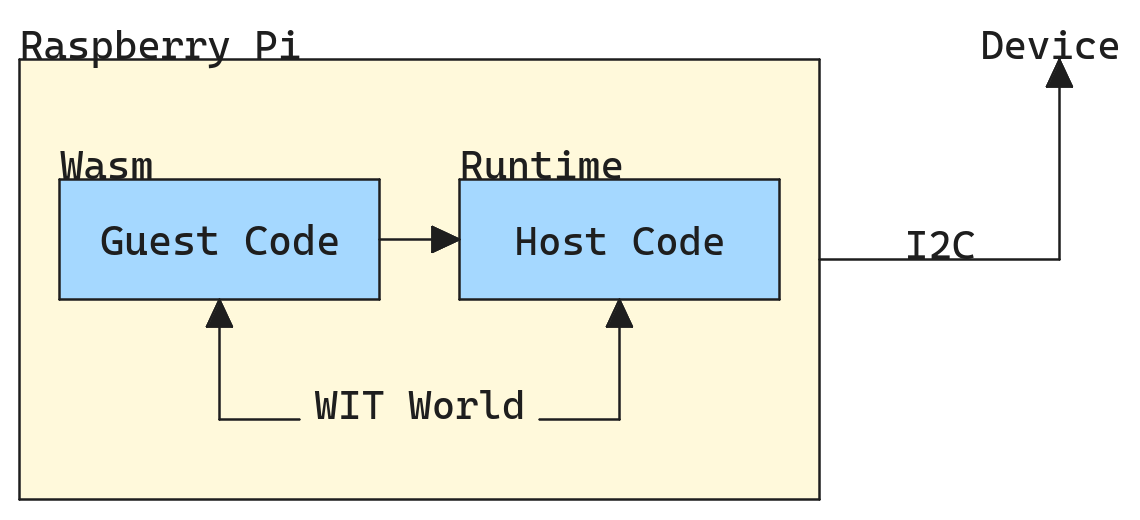
\includegraphics[width=0.5\textwidth]{figures/schema.png}
    \caption{Schematic overview of an implementation.}
    \label{fig:schematic}
\end{figure}

Conceptually, each implementation comes down to the schematic defined in figure~\ref{fig:schematic}. Only the guest code differs for each device. See chapter~\ref{chap:wasm} for an in-depth explanation.

% TODO: Hier foto's zetten van de verschillende setups

\section{Embedded driver development in Rust}
% [Native driver development, hoe gaat het te werk en de grote verschillen voor native development voor een gewone Pi en een microcontroller zoals de Pi Pico.]
Besides the implementation itself, two things are of significance to design a device driver in Rust. Namely, following the Embedded \gls{HAL} \gls{API}, see chapter~\ref{chap:hardware}, and supporting the desired target architecture.

Fortunately, Rust provides support for a great deal of platforms. Thus, building for ARM64 is as simple as providing the \texttt{--target aarch64-unknown-linux-gnu} flag. However, the RP2040 architecture needs special attention. For this, besides setting the \texttt{--target} flag with \texttt{thumbv6m-none-eabi}, we also need to provide a file called \texttt{memory.x}. 
This file is a linker script which specifies the memory layout of the target device, see section~\ref{sec:running}. Furthermore, the \gls{MCU} has only support for a \texttt{no\_std}.

\section{Embedded driver development in WebAssembly}
% [Om van native naar Wasm te gaan, wat moet er veranderen.]embedded-hal 0.2 vs 1.0 vermelden
Besides the considerations from the previous section, we now also need to keep the used runtime target platform support in mind. See section~\ref{sec:runtimes} for an overview. Furthermore, in this section, the different features of each runtime are also highlighted. These led to a vastly different implementation for both the host and the guest code.

\subsection{Wasmtime}

The guest is made into a component via the procedure specified in section~\ref{sec:guest}. The configured \gls{WIT} interface is the one specified in codefragment~\ref{code:wit}. 
Herein \texttt{wasi:i2c} is the proposal, as explained in chapter~\ref{chap:architecture}. Both displays are represented by the \texttt{screen} world, which needs both \texttt{i2c} and \texttt{delay} from the proposal. The HTS221 is mapped with the \texttt{sensor} world, that only needs \texttt{i2c}. Therefore, the former just includes the imports from \texttt{wasi:i2c}, while the latter only imports \texttt{i2c}.

The generated bindings have no way of knowing that they actually should follow the \texttt{embedded-hal} traits, for this the \href{https://github.com/Zelzahn/wasi-embedded-hal}{wasi-embedded-hal} crate is used.

On the side of the host, binding is done as described in section~\ref{sec:host}. Here, \texttt{wasi:i2c} is seen as a missing import, thus the \texttt{with} option is used with a data structure that implements the necessary traits.

\begin{listing}[h]
\begin{minted}[samepage]{rust}
package sketch:implementation;

interface hts {
    use wasi:i2c/i2c@0.2.0-draft.{i2c, error-code};

    get-temperature: func(connection: i2c) -> result<string, error-code>;
    get-humidity: func(connection: i2c) -> result<string, error-code>;
}

interface lcd {
    use wasi:i2c/i2c@0.2.0-draft.{i2c};
    use wasi:i2c/delay@0.2.0-draft.{delay};

    write: func(connection: i2c, delay: delay, message: string);
}

world sensor {
    import wasi:i2c/i2c@0.2.0-draft;

    export hts;
}

world screen {
    include wasi:i2c/imports@0.2.0-draft;

    export lcd;
}
\end{minted}
\caption{The \gls{WIT} interface to which guest and host bind.}
\label{code:wit}
\end{listing}

\subsection{WAMR}
% [vertellen dat ik in WAMR constrained was tot het doorgeven van simpele datatypes en dan maar met die globale connectie gewerkt heb]
As explained in section~\ref{sec:runtimes}, \gls{WAMR} is a lightweight runtime that, currently, has no support for preview 2. To sustain a pure Rust codebase, \href{https://github.com/bytecodealliance/wamr-rust-sdk}{WAMR Rust SDK} is used. This SDK provides Rust language bindings and support for passing integers and floats between the host and the guest. Note that strings can be passed via a conversion to a vector of the string code points.

As we can no longer use \gls{WIT}, nor pass a connection to the guest, we are enforced to greatly differ from the Wasmtime implementation. Therefore, we will focus us on the simpler 4-digit 7-segment display with the following conceptuel differences for \gls{WAMR}: The \gls{I2C} connection is kept global inside the host and there are now 4 arguments for the \texttt{write} function, one for each digit.

\subsection{Problems}
%TODO: Vertellen over gemerkte tekortkomingen aan WAMR, component model enzo
% Bvb. Is het mogelijk om Component Model voor MCU's te gebruiken
